% Submit
% https://edas.info/newPaper.php?c=34309
%Register a paper for 2026 IEEE Global Communications Conference: Selected Areas in Communications: E-Health

\documentclass[10pt,conference]{IEEEtran}
\IEEEoverridecommandlockouts
% The preceding line is only needed to identify funding in the first footnote. If that is unneeded, please comment it out.
\usepackage{algorithm}
\usepackage{algpseudocode}
\usepackage{cite}
\usepackage{amsmath,amssymb,amsfonts}

%\usepackage{algorithmic}
\usepackage{graphicx}
\usepackage{textcomp}
\usepackage{xcolor}
\usepackage{booktabs}
\usepackage{multirow}
\usepackage{siunitx}

\usepackage[caption=false]{subfig}
\usepackage[hyphens]{url}
\usepackage[hidelinks,bookmarks=false]{hyperref}
\usepackage{balance}
\usepackage{tabularx,multirow,booktabs,array}

%\usepackage{tikz}
%\usepackage{algorithm}
%\usepackage{algorithmic}



\usepackage{tikz}
\usetikzlibrary{shapes.geometric,arrows.meta,positioning,calc,fit,backgrounds,decorations.markings}
%\usetikzlibrary{arrows.meta,positioning,shapes,fit}
\usepackage{pgfplots}
\pgfplotsset{compat=1.18}
\usepgfplotslibrary{groupplots}

\def\BibTeX{{\rm B\kern-.05em{\sc i\kern-.025em b}\kern-.08em
    T\kern-.1667em\lower.7ex\hbox{E}\kern-.125emX}}

\pgfplotsset{
    every axis/.append style={
        font=\scriptsize,
        tick label style={font=\scriptsize},
        label style={font=\scriptsize},
        title style={font=\scriptsize},
        legend style={font=\scriptsize},
        grid=major,
        width=0.245\textwidth,
        height=0.17\textwidth,
        mark size=1.3pt,
        line width=0.8pt,
        xlabel near ticks,
        ylabel near ticks,
        legend cell align=left,
        legend style={
            draw=none,
            fill=none,
            at={(0.02,0.98)},
            anchor=north west
        }
    }
}


% ---------------------------------------------------------------------------
% Float spacing. Tightens the vertical gap between stacked figures so the
% results figures pack more densely and the bibliography pulls back onto p.6.
% IEEEtran defaults are floatsep 10.2pt, textfloatsep 18.6pt, abovecaptionskip 6pt.
%
% NOTCH 1 (active): moderate. Roughly one figure row reclaimed.
% NOTCH 2: aggressive. Uncomment the second block and comment out the first if
%          notch 1 leaves a reference stranded on the last page. Verified to
%          compile with zero overfull vboxes.
% ---------------------------------------------------------------------------
\makeatletter
% --- notch 1: moderate ---
\setlength{\floatsep}{5pt plus 2pt minus 1pt}
\setlength{\textfloatsep}{12pt plus 2pt minus 3pt}
\setlength{\dblfloatsep}{5pt plus 2pt minus 1pt}
\setlength{\dbltextfloatsep}{12pt plus 2pt minus 3pt}
\setlength{\abovecaptionskip}{4pt}
% --- notch 2: aggressive ---
% \setlength{\floatsep}{3pt plus 1pt minus 1pt}
% \setlength{\textfloatsep}{8pt plus 2pt minus 2pt}
% \setlength{\dblfloatsep}{3pt plus 1pt minus 1pt}
% \setlength{\dbltextfloatsep}{8pt plus 2pt minus 2pt}
% \setlength{\abovecaptionskip}{2pt}
\makeatother

\begin{document}

\title{Asynchronous Layer-Wise Weight Updating for Communication-Efficient Federated Learning in IoT Health Devices
\thanks{This work is supported by JSPS KAKENHI Grant Numbers
JP25K07743 and JP23K24905, Japan.}}

%


\author{
	\IEEEauthorblockN{
        Thomas Llamzon\IEEEauthorrefmark{1},
        Mostafa Fouda\IEEEauthorrefmark{2},
        Mohamed I. Ibrahem\IEEEauthorrefmark{3},
        Sherief Hashima\IEEEauthorrefmark{4}, and
        Zubair Md Fadlullah\IEEEauthorrefmark{1}
}
 
\IEEEauthorblockA{\IEEEauthorrefmark{1}Department of Computer Science, Western University, London, ON, Canada.}
\IEEEauthorblockA{\IEEEauthorrefmark{2}Department of Electrical and Computer Engineering, Idaho State University, Pocatello, ID, USA.}
\IEEEauthorblockA{\IEEEauthorrefmark{3}Department of
Cyber Systems Engineering, Augusta University, Augusta, GA, USA.}
\IEEEauthorblockA{\IEEEauthorrefmark{4}Computational Learning Theory Team, RIKEN-AIP, Fukuoka, Japan.}

Emails: tllamzon@uwo.ca, mfouda@ieee.org, mibrahem@augusta.edu,
Sherief.hashima@riken.jp, zfadlullah@ieee.org
\vspace{-0.3cm}
} 


\maketitle

\begin{abstract}
Federated Learning (FL) enables collaborative model training across distributed Internet of Things (IoT) health devices without centralizing sensitive patient data. However, standard synchronous FL suffers from high communication overhead, as clients upload the entire model parameters in each round, severely constraining bandwidth-limited IoT devices. This paper proposes a periodic asynchronous layer-wise update schedule that partitions model parameters into shallow and deep groups, transmitting shallow parameters every round and synchronizing deep parameters every K rounds. We evaluate this approach for ECG classification on the PTB-XL dataset using a 1D Convolutional Neural Network across centralized, synchronous, and asynchronous FL architectures. In a controlled 3-client, 4-round simulation, asynchronous FL with K = 2 reduces client upload volume by 49.70\% and total communication by 24.85\% with no measurable cost in accuracy. Across three random seeds under IID partitioning, asynchronous K = 2 reaches 83.18\% mean accuracy (standard deviation 0.76) against a synchronous FedAvg baseline of 82.68\% (standard deviation 0.98), a mean paired difference of 0.50 percentage points that is not statistically distinguishable from zero (p = 0.31). Under non-IID partitioning with a Dirichlet concentration of 0.5, a single run reaches 84.62\% against a synchronous baseline of 84.53\%. At K = 4, upload reduction reaches 74.55\% in exchange for a clear accuracy loss (79.21\% under IID, single run). These results demonstrate that periodic layer-wise scheduling can substantially reduce uplink communication cost in resource-constrained FL deployments while preserving acceptable model utility.
\end{abstract}

\begin{IEEEkeywords}
Federated Learning, IoT, ECG Classification, Communication Efficiency, Asynchronous Updates
\end{IEEEkeywords}


\section{Introduction}

Federated Learning (FL) enables collaborative model training across distributed Internet of Things (IoT) devices while preserving data privacy, making it suitable for healthcare applications such as wearable electrocardiogram (ECG) monitoring. In these settings, devices generate sensitive physiological signals that cannot be centralized due to privacy and regulatory constraints. FL addresses data locality by exchanging model parameters instead of raw data, but it introduces a major bottleneck, communication cost. Fig.~\ref{fig:privacy_fl} illustrates the privacy-preserving learning setting, where raw ECG data remain local and only scheduled model updates are communicated.

Standard FL, particularly Federated Averaging (FedAvg), follows a synchronous round-based protocol where clients download the global model, perform local training, and upload the complete updated model to the server. For deep ECG classifiers with millions of parameters, repeated full-model uploads dominate the cost of training. This is especially problematic for IoT health devices, where uplink bandwidth, energy, and connectivity are constrained.

%In addition to bandwidth constraints, communication inefficiency directly impacts energy consumption and system latency in IoT health deployments. Frequent uplink transmissions drain battery-operated wearable devices and increase training delay under intermittent connectivity. Moreover, network variability across devices introduces additional inefficiencies in synchronous protocols, where faster clients remain idle while waiting for slower participants. These limitations highlight the need for communication-aware learning strategies that reduce unnecessary transmissions without sacrificing model performance.

Communication inefficiency also affects energy consumption and latency in IoT health deployments, where frequent uplink transmissions draw on battery-powered devices and can increase training delay. This motivates communication-aware learning strategies that reduce unnecessary transmissions without sacrificing performance; we address the transmitted volume directly and treat the downstream energy and latency effects as motivation rather than as measured outcomes.

Two properties of deep networks make uniform synchronization wasteful. First, parameter mass is highly uneven: in our ECG classifier the two convolutional blocks nearest the input account for $0.60\%$ of all parameters, so the uplink cost is almost entirely attributable to the remaining layers. Second, networks exhibit layer-wise convergence heterogeneity, with shallow layers stabilizing early while deeper layers continue adapting, which means the deep group is also the group best able to tolerate delayed aggregation. Together these suggest synchronizing the small, foundational shallow group at every round and deferring the large, staleness-tolerant deep group.

A key inefficiency is that conventional FL treats all model layers uniformly as depicted in Fig.~\ref{fig:big_picture}. However, deep networks learn hierarchically. Shallow layers capture general low-level signal features, while deeper layers encode task-specific representations and classification boundaries. This motivates a layer-aware communication strategy where different parts of the model are synchronized at different temporal frequencies.


\begin{figure}[t]
\centering
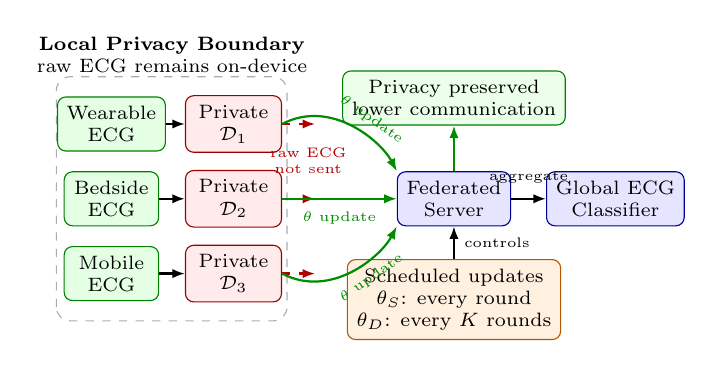
\begin{tikzpicture}[
font=\scriptsize,
box/.style={draw, rounded corners=3pt, align=center, minimum height=0.55cm},
device/.style={box, fill=green!10, draw=green!50!black, minimum width=1.20cm},
data/.style={box, fill=red!8, draw=red!60!black, minimum width=1.22cm},
server/.style={box, fill=blue!10, draw=blue!60!black, minimum width=1.30cm},
sched/.style={box, fill=orange!12, draw=orange!70!black, minimum width=2.15cm},
note/.style={box, fill=green!8, draw=green!50!black, minimum width=2.05cm},
arr/.style={-{Latex[length=1.6mm]}, thick},
safe/.style={-{Latex[length=1.6mm]}, thick, green!55!black},
blocked/.style={-{Latex[length=1.6mm]}, thick, red!70!black, dashed}
]

% Privacy area
\draw[gray!65, dashed, rounded corners=5pt]
(-3.75,-1.55) rectangle (-0.82,1.55);
\node[align=center] at (-2.28,1.83)
{\textbf{Local Privacy Boundary}\\raw ECG remains on-device};

% Devices and private data
\node[device] (w1) at (-3.05,0.95) {Wearable\\ECG};
\node[device] (w2) at (-3.05,0.00) {Bedside\\ECG};
\node[device] (w3) at (-3.05,-0.95) {Mobile\\ECG};

\node[data] (d1) at (-1.50,0.95) {Private\\$\mathcal{D}_1$};
\node[data] (d2) at (-1.50,0.00) {Private\\$\mathcal{D}_2$};
\node[data] (d3) at (-1.50,-0.95) {Private\\$\mathcal{D}_3$};

\draw[arr] (w1) -- (d1);
\draw[arr] (w2) -- (d2);
\draw[arr] (w3) -- (d3);

% Server side
\node[server] (srv) at (1.30,0.00) {Federated\\Server};
\node[server] (clf) at (3.35,0.00) {Global ECG\\Classifier};

\node[note] (benefit) at (1.30,1.28)
{Privacy preserved\\lower communication};

\node[sched] (sch) at (1.30,-1.28)
{Scheduled updates\\$\theta_S$: every round\\$\theta_D$: every $K$ rounds};

% Raw data blocked, short dead-end arrows
\draw[blocked] (d1.east) -- ++(0.42,0);
\draw[blocked] (d2.east) -- ++(0.42,0);
\draw[blocked] (d3.east) -- ++(0.42,0);
\node[red!70!black, font=\tiny, align=center] at (-0.55,0.48)
{raw ECG\\not sent};

% Model update arrows, routed clearly
\draw[safe] (d1.east) .. controls (-0.25,1.28) and (0.38,0.72) ..
node[pos=0.58, above, sloped, font=\tiny]{$\theta$ update} (srv.north west);

\draw[safe] (d2.east) -- 
node[midway, below, yshift=-1pt, font=\tiny]{$\theta$ update} (srv.west);

\draw[safe] (d3.east) .. controls (-0.25,-1.28) and (0.38,-0.72) ..
node[pos=0.58, below, sloped, font=\tiny]{$\theta$ update} (srv.south west);

% Scheduling relation and aggregation
\draw[arr] (sch.north) -- node[right, font=\tiny]{controls} (srv.south);
\draw[arr] (srv.east) -- node[above, font=\tiny, yshift=2pt]{aggregate} (clf.west);

% Benefits connect to server, no overlap
\draw[arr, green!55!black] (srv.north) -- (benefit.south);

\end{tikzpicture}
\caption{Privacy-preserving federated learning for IoT health monitoring, where raw ECG records remain on local devices and only scheduled model updates are transmitted to the server.}
\label{fig:privacy_fl}
\end{figure}


% \begin{figure}[t]
% \centering
% \begin{tikzpicture}[
% font=\scriptsize,
% node distance=0.9cm,
% box/.style={draw, rounded corners, align=center, minimum width=1.45cm, minimum height=0.55cm},
% server/.style={box, fill=blue!10},
% client/.style={box, fill=green!10},
% shallow/.style={box, fill=orange!15},
% deep/.style={box, fill=red!10},
% arr/.style={->, thick}
% ]
% \node[server] (srv) at (0,0) {FL Server\\Global Model};
% \node[client] (c1) at (-2.7,-1.6) {ECG IoT\\Client 1};
% \node[client] (c2) at (0,-1.9) {ECG IoT\\Client 2};
% \node[client] (c3) at (2.7,-1.6) {ECG IoT\\Client 3};

% \node[shallow] (s) at (-1.2,1.2) {Shallow Layers\\sync every round};
% \node[deep] (d) at (1.4,1.2) {Deep Layers\\sync every $K$ rounds};

% \draw[arr] (srv) -- node[left]{full model} (c1);
% \draw[arr] (srv) -- node[right]{full model} (c2);
% \draw[arr] (srv) -- node[right]{full model} (c3);

% \draw[arr, dashed] (c1) -- node[left]{partial/full upload} (srv);
% \draw[arr, dashed] (c2) -- (srv);
% \draw[arr, dashed] (c3) -- (srv);

% \draw[arr] (srv) -- (s);
% \draw[arr] (srv) -- (d);

% \node[align=center] at (0,-3.0) {Layer-wise temporal scheduling reduces uplink cost while preserving standard FL operation.};
% \end{tikzpicture}
% \caption{Big-picture view of the proposed asynchronous layer-wise FL framework for IoT health devices.}
% \label{fig:big_picture}
% \end{figure}


\begin{figure}[t]
\centering
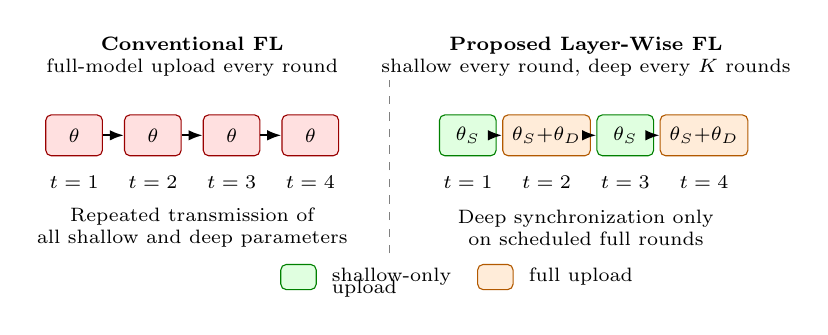
\begin{tikzpicture}[
font=\scriptsize,
round/.style={draw, rounded corners=2pt, minimum width=0.72cm, minimum height=0.52cm, align=center},
full/.style={round, fill=red!12, draw=red!60!black},
partial/.style={round, fill=green!12, draw=green!50!black},
deep/.style={round, fill=orange!15, draw=orange!70!black},
label/.style={align=center},
arr/.style={-{Latex[length=1.8mm]}, thick}
]

% Title labels
\node[label] at (-2.5,1.45) {\textbf{Conventional FL}\\full-model upload every round};
\node[label] at (2.5,1.45) {\textbf{Proposed Layer-Wise FL}\\shallow every round, deep every $K$ rounds};

% Conventional timeline
\node[full] (f1) at (-4.0,0.45) {$\theta$};
\node[full] (f2) at (-3.0,0.45) {$\theta$};
\node[full] (f3) at (-2.0,0.45) {$\theta$};
\node[full] (f4) at (-1.0,0.45) {$\theta$};

\draw[arr] (f1) -- (f2);
\draw[arr] (f2) -- (f3);
\draw[arr] (f3) -- (f4);

\node[label] at (-4.0,-0.15) {$t=1$};
\node[label] at (-3.0,-0.15) {$t=2$};
\node[label] at (-2.0,-0.15) {$t=3$};
\node[label] at (-1.0,-0.15) {$t=4$};

\node[label] at (-2.5,-0.72) {Repeated transmission of\\all shallow and deep parameters};

% Proposed timeline
\node[partial] (p1) at (1.0,0.45) {$\theta_S$};
\node[deep]    (p2) at (2.0,0.45) {$\theta_S{+}\theta_D$};
\node[partial] (p3) at (3.0,0.45) {$\theta_S$};
\node[deep]    (p4) at (4.0,0.45) {$\theta_S{+}\theta_D$};

\draw[arr] (p1) -- (p2);
\draw[arr] (p2) -- (p3);
\draw[arr] (p3) -- (p4);

\node[label] at (1.0,-0.15) {$t=1$};
\node[label] at (2.0,-0.15) {$t=2$};
\node[label] at (3.0,-0.15) {$t=3$};
\node[label] at (4.0,-0.15) {$t=4$};

\node[label] at (2.5,-0.72) {Deep synchronization only\\on scheduled full rounds};

% Divider
\draw[dashed, gray] (0,-1.05) -- (0,1.15);

% Legend
\node[partial, minimum width=0.45cm, minimum height=0.32cm] at (-1.15,-1.35) {};
\node[anchor=west] at (-0.85,-1.35) {shallow-only};
\node[anchor=west] at (-0.85,-1.5) {upload};

\node[deep, minimum width=0.45cm, minimum height=0.32cm] at (1.35,-1.35) {};
\node[anchor=west] at (1.65,-1.35) {full upload};

\end{tikzpicture}
\caption{Conceptual comparison between conventional full-model FL and the proposed periodic layer-wise update strategy.}
\label{fig:big_picture}
\end{figure}

%From a learning perspective, deep neural networks exhibit layer-wise convergence heterogeneity. Early convolutional layers tend to stabilize rapidly as they capture general signal characteristics, while deeper layers continue adapting to task-specific patterns. This suggests that enforcing uniform synchronization frequency across all layers is suboptimal. Instead, communication schedules can be aligned with the intrinsic learning dynamics of different parameter groups.

In this paper we study the simplest realizable form of layer-wise update scheduling: a fixed partition of the model into shallow and deep parameter groups, with shallow layers synchronized every round and deep layers every $K$ rounds. Unlike adaptive layer-wise schemes, the partition and the interval are set in advance, so the server maintains no per-layer statistics and the method reduces to a scheduling rule over unmodified FedAvg. We characterize the resulting communication and accuracy behaviour on PTB-XL ECG classification under IID and non-IID partitions. At $K=2$ upload cost falls by 49.70\% with accuracy statistically indistinguishable from synchronous FL over three seeds, and at $K=4$ upload reduction reaches 74.55\% with a clear accuracy cost.

The remainder of this paper is organized as follows. Section II reviews related work. Section III presents the considered system model and problem formulation. Section IV describes the proposed methodology and algorithm. Section V provides complexity analysis. Section VI presents performance evaluation. Section VII concludes the paper.
\section{Related Work}

Federated Learning (FL) was popularized by McMahan et al. \cite{mcmahan2017} through the Federated Averaging (FedAvg) algorithm, where a central server coordinates training by aggregating locally updated client models. Subsequent work by Yang et al. \cite{yang2019} formalized the FL paradigm into horizontal, vertical, and transfer settings. Healthcare IoT applications, such as ECG monitoring, fall under horizontal FL, where devices share the same feature space but operate on different patient data distributions.

A major limitation of FL is communication overhead. Konečný et al. \cite{konecny2016} showed that communication rounds dominate overall training time, particularly in heterogeneous environments with varying device and network capabilities. To address this, prior work has focused on reducing the size of transmitted updates. Kone\v{c}n\'y et al. \cite{konecny2016strategies} introduced structured and sketched updates, including sparse parameter selection, probabilistic quantization, and low-rank factorization, demonstrating substantial reductions in uplink volume; these techniques are surveyed in \cite{hartmann2018}. While compression-based approaches \cite{lin2018deepgradient} and optimization-aware methods \cite{reddi2021adaptive,karimireddy2020scaffold} have been extensively studied for reducing communication overheads, the aforementioned approaches apply uniform compression across all model layers and do not exploit the hierarchical structure of deep networks.

An alternative direction is to modify the computation architecture. Yuan et al. \cite{yuan2020} proposed a split learning approach for healthcare IoT, where shallow layers are executed on-device and deeper layers are offloaded to a central server. Combined with sparsification of exchanged activations and gradients, this method achieves substantial communication reduction while maintaining accuracy. However, it changes the standard FL architecture and retains synchronous round assumptions, without adapting communication frequency across different parts of the model.

Another line of work focuses on relaxing synchronization constraints. Asynchronous FL methods \cite{xie2019asynchronous} allow clients to update the server without strict round barriers, improving system efficiency under heterogeneous conditions. While effective in reducing idle time, these approaches typically treat the model as a single parameter block and do not differentiate between layers in terms of communication frequency. Recent surveys \cite{tariq2024} further highlight that communication efficiency remains a central challenge in IoT and edge FL deployments, especially under non-IID data and unreliable networks. Recent work has explored layer-wise adaptive federated learning \cite{xu2021layerwise}, but without incorporating temporal scheduling of parameter updates within standard FL rounds.

Layer-wise scheduling itself is not new. FedLAMA \cite{xu2021layerwise} adjusts the aggregation interval in a layer-wise manner, jointly considering model discrepancy and communication cost, and maintains per-layer statistics at the server to do so. Despite these advances, layer-wise scheduling has so far been posed as a runtime adaptation problem, in which per-layer synchronization intervals are derived from measured model discrepancy and maintained by the server. We ask a narrower question: how much of the benefit survives when the schedule is fixed in advance and requires no measurement, no coordination, and no per-layer state at all. Our contribution is therefore not the idea of layer-wise scheduling but a characterization of its simplest realizable form, a static two-group partition chosen by parameter mass with a single constant interval, evaluated in a resource-constrained IoT health setting.

\section{Considered System Model and Problem Formulation}

We consider an IoT healthcare FL system with one coordinating server and $N$ distributed ECG clients. Each client $i$ stores a private local dataset $\mathcal{D}_i=\{(\mathbf{x}_{i,j},y_{i,j})\}_{j=1}^{n_i}$, where $\mathbf{x}_{i,j}\in\mathbb{R}^{5000\times 12}$ denotes a 12-lead ECG segment and $y_{i,j}\in\{0,1\}$ denotes the binary label, normal or abnormal. Raw ECG records remain local and are never transmitted to the server.

\begin{figure}[t]
\centering
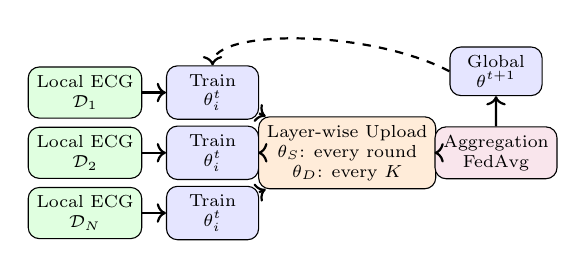
\begin{tikzpicture}[
font=\scriptsize,
scale=0.9,
transform shape,
box/.style={draw, rounded corners, align=center, minimum width=1.3cm, minimum height=0.5cm},
data/.style={box, fill=green!12},
model/.style={box, fill=blue!10},
sched/.style={box, fill=orange!15},
server/.style={box, fill=purple!10},
arr/.style={->, thick}
]

% Left side (data)
\node[data] (d1) at (-2.4,0) {Local ECG\\$\mathcal{D}_1$};
\node[data] (d2) at (-2.4,-0.85) {Local ECG\\$\mathcal{D}_2$};
\node[data] (d3) at (-2.4,-1.7) {Local ECG\\$\mathcal{D}_N$};

% Local training
\node[model] (m1) at (-0.6,0) {Train\\$\theta_i^t$};
\node[model] (m2) at (-0.6,-0.85) {Train\\$\theta_i^t$};
\node[model] (m3) at (-0.6,-1.7) {Train\\$\theta_i^t$};

% Upload block (shorter text)
\node[sched] (up) at (1.3,-0.85)
{Layer-wise Upload\\$\theta_S$: every round\\$\theta_D$: every $K$};

% Server
\node[server] (agg) at (3.4,-0.85)
{Aggregation\\FedAvg};

% Global model
\node[model] (global) at (3.4,0.3)
{Global\\$\theta^{t+1}$};

% Connections
\draw[arr] (d1) -- (m1);
\draw[arr] (d2) -- (m2);
\draw[arr] (d3) -- (m3);

\draw[arr] (m1) -- (up);
\draw[arr] (m2) -- (up);
\draw[arr] (m3) -- (up);

\draw[arr] (up) -- (agg);
\draw[arr] (agg) -- (global);

% Feedback (tight curve)
\draw[arr, dashed]
(global.west) .. controls (1.6,0.9) and (-0.6,0.9) .. (m1.north);

\end{tikzpicture}
\caption{Considered system model for asynchronous layer-wise FL.}
\label{fig:system_tikz}
\end{figure}

Let $\boldsymbol{\theta}$ denote the full model parameters. The conventional FL objective is
\begin{equation}
\min_{\boldsymbol{\theta}} F(\boldsymbol{\theta})
=
\sum_{i=1}^{N}\frac{n_i}{n}F_i(\boldsymbol{\theta}),
\quad
F_i(\boldsymbol{\theta})
=
\frac{1}{n_i}\sum_{j=1}^{n_i}
\ell(f_{\boldsymbol{\theta}}(\mathbf{x}_{i,j}),y_{i,j}),
\end{equation}
where $n=\sum_i n_i$, $F_i$ is the empirical local loss, and $\ell(\cdot)$ is the binary cross-entropy loss. The global objective captures collaborative learning across heterogeneous clients, where each local distribution may differ due to patient-specific characteristics, acquisition devices, or noise conditions. In practical IoT healthcare deployments, such statistical heterogeneity leads to non-IID data distributions~\cite{li2020federated,wang2020tackling}, which are known to slow convergence and destabilize federated optimization. Therefore, any communication-efficient strategy must maintain robustness under both IID and non-IID conditions.

In standard synchronous FL, each participating client uploads the full parameter vector $\boldsymbol{\theta}_i^t$ at every round. The communication cost therefore scales with the full model size. In contrast, we partition the model into shallow and deep components,
\begin{equation}
\boldsymbol{\theta}=(\boldsymbol{\theta}_S,\boldsymbol{\theta}_D),
\end{equation}
where $\boldsymbol{\theta}_S$ contains early convolutional layers and $\boldsymbol{\theta}_D$ contains later convolutional and fully connected layers. The goal is to reduce uplink communication while preserving model utility. This gives the following communication-aware design problem:
\begin{equation}
\label{eq:uplink_budget}
\min_{\{\boldsymbol{\theta}^t\}_{t=1}^{T}}
F(\boldsymbol{\theta}^T)
\quad
\text{s.t.}
\quad
\sum_{t=1}^{T}C_{\text{up}}(t)\leq B,
\end{equation}
where $B$ is the available uplink budget. This formulation follows standard federated optimization frameworks \cite{mcmahan2017,li2020federated}.  \noindent
The formulation in \eqref{eq:uplink_budget} implicitly assumes that all model parameters contribute equally to the communication cost, which is not the case in deep neural networks. In our ECG classifier the two convolutional blocks nearest the input hold $0.60\%$ of the parameters, while the remaining layers hold $99.40\%$. Uplink cost is therefore almost entirely determined by the deep group, and synchronizing the shallow group is nearly free. This asymmetry, not convergence speed, is what makes a differentiated schedule worthwhile: sending the inexpensive group at every round and the expensive group periodically is the only partition that yields a meaningful reduction in uplink volume.

Convergence heterogeneity enters as a separate question, namely which group can tolerate being stale. Prior work on feature transferability \cite{yosinski2014} shows that early layers learn general representations while deeper layers specialize for the target task. Deep layers encode slower-changing, task-specific structure and therefore tolerate delayed aggregation, whereas the shallow layers form the shared feature extractor that every deep layer builds upon. Keeping that extractor consistent across clients at every round is what keeps the periodically aggregated deep layers mutually coherent. The two arguments are complementary: parameter mass determines which group is expensive to send, and staleness tolerance determines which group can afford to wait. Rather than solving this constrained problem directly, we adopt a periodic layer-wise schedule that controls when deep parameters are transmitted. The above formulation highlights the trade-off between model accuracy and communication cost. Reducing communication by limiting parameter transmission may introduce staleness in the global model, particularly for deep parameters that are not updated every round. The design challenge is therefore to determine a scheduling strategy that minimizes communication while preserving sufficient update frequency for critical model components.


\section{Proposed Methodology}

We use the term \emph{asynchronous} in a layer-wise rather than a client-wise sense, and the distinction matters. Conventional asynchronous FL removes the round barrier between clients, allowing each client to update the server independently and at its own pace. Our scheme retains the standard synchronous round structure and full client participation; what varies asynchronously is \emph{which parameter groups are synchronized in a given round}. Shallow parameters are aggregated every round, deep parameters every $K$ rounds, so different parts of the model are updated on different schedules and the deep group carries a bounded staleness of at most $K-1$ rounds. The method is therefore complementary to client-wise asynchrony rather than an instance of it, and the two could be combined.

This section describes the experimental framework and the proposed asynchronous layer-wise scheduling strategy. The goal is to isolate the impact of temporal layer-wise communication on learning performance and communication cost.

\subsection{Experimental Design}

We compare three training architectures, centralized training, synchronous FL, and asynchronous layer-wise FL. The centralized setup provides a non-federated reference point, synchronous FL serves as the FedAvg baseline, and the asynchronous variant applies the proposed periodic scheduling. All settings use the same dataset, preprocessing, model architecture, optimizer, and training budget.

All runs fix the Python, NumPy, and PyTorch random seeds and pin the PyTorch intra-op thread count; a single training step was verified bitwise identical at 1, 2, 3, 4, 8, and 10 threads, so results are invariant to host CPU load and core count. For a given seed the synchronous and asynchronous runs consume identical partitions and have bitwise identical round-zero checkpoints, so the schedules are compared from the same initialization on the same data. The IID synchronous and $K=2$ configurations are repeated at three seeds; the rest are single runs.

\subsection{Dataset and Model}

Experiments use the PTB-XL dataset \cite{wagner2020}, a 12-lead ECG benchmark with 21,799 records sampled at 500 Hz. Each input is a 10-second ECG signal of shape $(5000,12)$. The task is binary classification between Normal and Abnormal rhythms. Folds 1--9 are used for training and fold 10 is used for testing.

The ECGCNN model contains 37,130,657 parameters, approximately 148.5 MB. The shallow group consists of \texttt{conv1}, \texttt{bn1}, \texttt{conv2}, and \texttt{bn2}, totaling 897,936 bytes, or 0.60\% of the model. The deep group consists of \texttt{conv3}, \texttt{bn3}, \texttt{conv4}, \texttt{bn4}, \texttt{fc1}, \texttt{fc2}, and \texttt{fc3}, totaling 147,628,564 bytes, or 99.40\%. This highly imbalanced partition is useful for testing whether infrequent deep synchronization can reduce communication without collapsing accuracy.

\subsection{Federated Setup}

The federated setting uses three simulated clients. Training runs for four communication rounds, with one participating client per round and one local epoch per selected client. Local training uses Adam with learning rate $10^{-3}$ and batch size 32. Both IID and non-IID partitions are evaluated. The non-IID split uses a Dirichlet distribution with $\alpha=0.5$.

\subsection{Asynchronous Layer-Wise Schedule}

At round $t$, let $\mathcal{P}_t$ be the participating client set. The server computes sample-weighted aggregation for shallow and deep parameters as
\begin{equation}
\operatorname{Agg}_S^t =
\sum_{i\in\mathcal{P}_t}w_i^t\boldsymbol{\theta}_{S,i}^t,
\quad
\operatorname{Agg}_D^t =
\sum_{i\in\mathcal{P}_t}w_i^t\boldsymbol{\theta}_{D,i}^t,
\end{equation}
where $w_i^t=n_i/\sum_{j\in\mathcal{P}_t}n_j$.

The shallow group is updated every round:
\begin{equation}
\boldsymbol{\theta}_S^{t+1}=\operatorname{Agg}_S^t.
\end{equation}
The deep group is updated periodically:
\begin{equation}
\boldsymbol{\theta}_D^{t+1}=
\begin{cases}
\operatorname{Agg}_D^t, & t \bmod K=0,\\
\widehat{\boldsymbol{\theta}}_D^t, & \text{otherwise},
\end{cases}
\end{equation}
where $\widehat{\boldsymbol{\theta}}_D^t$ is the cached deep parameter state from the most recent full update.

The uplink cost at round $t$ is
\begin{equation}
C_{\text{up}}(t)=|\mathcal{P}_t|
\left(
|\boldsymbol{\theta}_S|
+
|\boldsymbol{\theta}_D|\mathbb{I}[t\bmod K=0]
\right),
\end{equation}
while the downlink cost is
\begin{equation}
C_{\text{down}}(t)=|\mathcal{P}_t|
\left(
|\boldsymbol{\theta}_S|+|\boldsymbol{\theta}_D|
\right).
\end{equation}

\noindent
The proposed scheduling mechanism introduces a trade-off between communication efficiency and parameter freshness. While shallow layers are continuously updated, deep parameters may become stale between full synchronization rounds. However, since shallow layers stabilize feature extraction, they can maintain consistent intermediate representations even when deep parameters are temporarily outdated. This results in a form of partial consistency, where feature quality is preserved while classification layers are intermittently refined. The effectiveness of this mechanism depends on the scheduling period $K$ and the relative contribution of each parameter group to the overall model. %The proposed schedule introduces controlled staleness in deep parameters. While this reduces communication, it may delay convergence if deep representations become outdated. However, shallow layers provide continuous updates that stabilize early feature extraction, partially mitigating the impact of deep-layer staleness. This design leverages the hierarchical nature of deep models to balance communication efficiency and learning progress.

\begin{algorithm}[t]
\caption{Periodic Asynchronous Layer-Wise FL}
\label{alg:async_layerwise}
\begin{algorithmic}[1]
\State Initialize global model $\boldsymbol{\theta}^{0}=(\boldsymbol{\theta}_{S}^{0},\boldsymbol{\theta}_{D}^{0})$
\State Initialize cached deep parameters $\widehat{\boldsymbol{\theta}}_{D}^{0}\gets\boldsymbol{\theta}_{D}^{0}$
\For{$t=1,\ldots,T$}
    \State Server selects participating clients $\mathcal{P}_{t}$
    \State Server broadcasts full model $\boldsymbol{\theta}^{t}$
    \For{each client $i\in\mathcal{P}_{t}$}
        \State Client trains locally for one epoch to obtain $\boldsymbol{\theta}_{i}^{t}$
        \If{$t \bmod K = 0$}
            \State Client uploads $(\boldsymbol{\theta}_{S,i}^{t},\boldsymbol{\theta}_{D,i}^{t})$
        \Else
            \State Client uploads $\boldsymbol{\theta}_{S,i}^{t}$ only
        \EndIf
    \EndFor
    \State Aggregate shallow parameters:
    \Statex \hspace{\algorithmicindent}$\boldsymbol{\theta}_{S}^{t+1}\gets
    \sum_{i\in\mathcal{P}_{t}} w_i^t \boldsymbol{\theta}_{S,i}^{t}$
    \If{$t \bmod K = 0$}
        \State Aggregate deep parameters:
        \Statex \hspace{\algorithmicindent}$\boldsymbol{\theta}_{D}^{t+1}\gets
        \sum_{i\in\mathcal{P}_{t}} w_i^t \boldsymbol{\theta}_{D,i}^{t}$
        \State Update cache $\widehat{\boldsymbol{\theta}}_{D}^{t+1}\gets\boldsymbol{\theta}_{D}^{t+1}$
    \Else
        \State Reuse cached deep parameters:
        \Statex \hspace{\algorithmicindent}$\boldsymbol{\theta}_{D}^{t+1}\gets\widehat{\boldsymbol{\theta}}_{D}^{t}$
    \EndIf
    \State Form updated global model $\boldsymbol{\theta}^{t+1}=(\boldsymbol{\theta}_{S}^{t+1},\boldsymbol{\theta}_{D}^{t+1})$
\EndFor
\end{algorithmic}
\end{algorithm}



\section{Communication and Complexity Analysis}

Let $P_S=|\boldsymbol{\theta}_S|$ and $P_D=|\boldsymbol{\theta}_D|$ denote the number of transmitted bytes for shallow and deep parameters, respectively. Let $M_t=|\mathcal{P}_t|$ be the number of participating clients at round $t$. In synchronous FL, each client uploads the full model every round, giving
\begin{equation}
C_{\text{sync}}^{\text{up}}
=
\sum_{t=1}^{T} M_t(P_S+P_D).
\end{equation}

For the proposed asynchronous schedule, deep parameters are uploaded only on full rounds. Thus,
\begin{equation}
C_{\text{async}}^{\text{up}}
=
\sum_{t=1}^{T}M_tP_S
+
\sum_{t=1}^{T}M_tP_D\mathbb{I}[t\bmod K=0].
\end{equation}
If $M_t=M$ for all rounds and $K$ divides $T$, this simplifies to
\begin{equation}
C_{\text{async}}^{\text{up}}
=
MT P_S
+
M\frac{T}{K}P_D.
\end{equation}
The corresponding uplink reduction relative to synchronous FL is
\begin{equation}
\rho_{\text{up}}
=
1-
\frac{P_S+\frac{1}{K}P_D}{P_S+P_D}.
\end{equation}

\noindent
From an optimization perspective, the periodic omission of deep parameter updates can be interpreted as a form of delayed gradient aggregation. While such delays may slow convergence, their impact is mitigated when the delayed components correspond to parameters with slower update dynamics. In the considered ECGCNN architecture, deep layers evolve more gradually compared to shallow layers, making them more tolerant to reduced update frequency. This partially explains why moderate scheduling periods, such as $K=2$, maintain accuracy while achieving significant communication savings.

Since $P_D\gg P_S$ in the ECGCNN model, the reduction is approximately $1-1/K$. Therefore, $K=2$ yields close to 50\% upload reduction, while $K=4$ yields close to 75\% upload reduction. This matches the empirical reductions of 49.70\% and 74.55\%, respectively.

The computational complexity of local training is unchanged because each client trains the full model after receiving the global model. If one local epoch costs $\mathcal{O}(n_iP)$ for client $i$, where $P=P_S+P_D$, then both synchronous and asynchronous FL have the same local training order. The main reduction is therefore not in floating-point computation but in uplink transmission. On the server side, aggregation cost is reduced during shallow-only rounds from $\mathcal{O}(MP)$ to $\mathcal{O}(MP_S)$, while full rounds retain $\mathcal{O}(MP)$ complexity. Thus, the proposed method reduces both communication load and partial server aggregation cost without changing client-side model execution.

From a system perspective, the reduction in uplink volume suggests several potential benefits that we did not measure. Lower peak uplink demand during shallow-only rounds may reduce contention in multi-client deployments, and fewer transmitted bytes may reduce the energy spent on radio activity in battery-powered devices. We note these as expected consequences rather than findings. Our evaluation measures transmitted bytes only; we did not measure device power draw, wall-clock latency, packet loss, or behaviour under unstable network conditions, and byte savings alone do not straightforwardly predict energy savings, since radio startup and association overhead can dominate the per-transmission energy cost.

\section{Performance Evaluation}

This section evaluates the proposed asynchronous layer-wise FL scheme in terms of accuracy and communication cost. We compare centralized training, synchronous FL, and the proposed method under both IID and non-IID data distributions. All experiments use identical model architecture, training budget, and hyperparameters to isolate the effect of the scheduling mechanism.

\subsection{Centralized and Synchronous Baselines}

The centralized CNN achieves 84.08\% test accuracy with loss 0.3267 after four epochs, establishing a non-federated reference point. We note that some federated configurations exceed this value, so it is a reference rather than a bound. Fig.~\ref{fig:centralized} shows stable convergence, with training and validation curves indicating that the model effectively captures the ECG classification task.

\begin{figure}[!t]
\centering
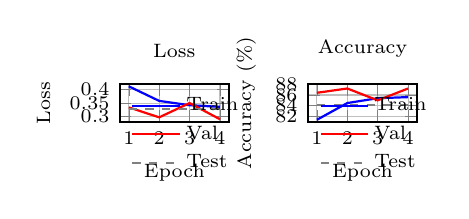
\begin{tikzpicture}
\begin{groupplot}[
    group style={group size=2 by 1, horizontal sep=1.0cm},
    xlabel={Epoch},
]
\nextgroupplot[title={Loss}, ylabel={Loss}, ymin=0.28, ymax=0.42]
\addplot[blue] coordinates {(1,0.412) (2,0.358) (3,0.342) (4,0.336)};
\addplot[red] coordinates {(1,0.334) (2,0.297) (3,0.350) (4,0.290)};
\addplot[gray, dashed] coordinates {(1,0.3267) (4,0.3267)};
\legend{Train, Val, Test}

\nextgroupplot[title={Accuracy}, ylabel={Accuracy (\%)}, ymin=81, ymax=88]
\addplot[blue] coordinates {(1,81.4) (2,84.5) (3,85.4) (4,85.6)};
\addplot[red] coordinates {(1,86.4) (2,87.2) (3,85.0) (4,87.2)};
\addplot[gray, dashed] coordinates {(1,84.08) (4,84.08)};
\legend{Train, Val, Test}
\end{groupplot}
\end{tikzpicture}
\caption{Centralized training curves.}
\label{fig:centralized}
\end{figure}

Under IID partitioning, synchronous FL achieves $82.68 \pm 0.98\%$ accuracy over three seeds (81.85\%, 82.44\%, 83.76\%); the run shown in Fig.~\ref{fig:sync_iid} reaches 81.85\% at loss 0.4015. Under non-IID partitioning with Dirichlet $\alpha=0.5$, a single run achieves 84.53\% accuracy with loss 0.3634, as shown in Fig.~\ref{fig:sync_noniid}. The comparable performance under non-IID in this setting is plausibly due to the small number of clients and moderate heterogeneity, but with a single run per partitioning scheme we cannot separate that explanation from seed variation, which alone spans 1.91 percentage points under IID.

\begin{figure}[!t]
\centering
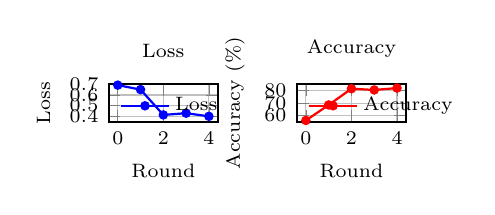
\begin{tikzpicture}
\begin{groupplot}[group style={group size=2 by 1, horizontal sep=1cm}, xlabel={Round}]
\nextgroupplot[title={Loss}, ylabel={Loss}, ymin=0.35, ymax=0.70]
\addplot[blue, mark=*] coordinates {(0,0.691) (1,0.650) (2,0.415) (3,0.431) (4,0.402)};
\legend{Loss}

\nextgroupplot[title={Accuracy}, ylabel={Accuracy (\%)}, ymin=55, ymax=85]
\addplot[red, mark=*] coordinates {(0,56.2) (1,68.5) (2,81.4) (3,80.4) (4,81.9)};
\legend{Accuracy}
\end{groupplot}
\end{tikzpicture}

\caption{Synchronous FL under IID partitioning.}
\label{fig:sync_iid}
\end{figure}

\begin{figure}[!t]
\centering
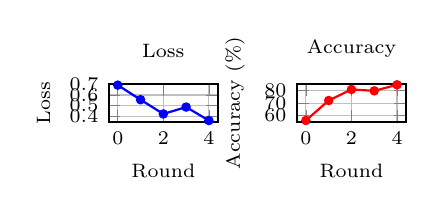
\begin{tikzpicture}
\begin{groupplot}[group style={group size=2 by 1}, xlabel={Round}]
\nextgroupplot[title={Loss}, ylabel={Loss}, ymin=0.35, ymax=0.70]
\addplot[blue, mark=*] coordinates {(0,0.691) (1,0.556) (2,0.424) (3,0.488) (4,0.363)};

\nextgroupplot[title={Accuracy}, ylabel={Accuracy (\%)}, ymin=55, ymax=85]
\addplot[red, mark=*] coordinates {(0,56.2) (1,72.0) (2,80.8) (3,79.7) (4,84.5)};
\end{groupplot}
\end{tikzpicture}
\caption{Synchronous FL under non-IID partitioning.}
\label{fig:sync_noniid}
\end{figure}

In both cases, full-model synchronization results in approximately 3.4 GB total communication, highlighting the inefficiency of transmitting all parameters at every round.

\subsection{Asynchronous FL Results}

The case $K=1$ reduces to standard synchronous FL and achieves comparable performance, validating the correctness of the implementation, as shown in Fig.~\ref{fig:async_k1}.

\begin{figure}[!t]
\centering
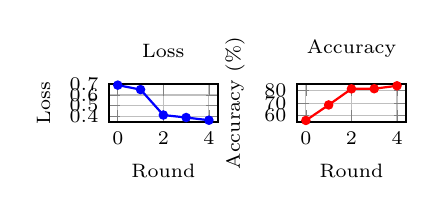
\begin{tikzpicture}
\begin{groupplot}[group style={group size=2 by 1}, xlabel={Round}]
\nextgroupplot[title={Loss}, ylabel={Loss}, ymin=0.35, ymax=0.70]
\addplot[blue, mark=*] coordinates {(0,0.691) (1,0.650) (2,0.414) (3,0.391) (4,0.366)};

\nextgroupplot[title={Accuracy}, ylabel={Accuracy (\%)}, ymin=55, ymax=85]
\addplot[red, mark=*] coordinates {(0,56.2) (1,68.5) (2,81.3) (3,81.4) (4,83.7)};
\end{groupplot}
\end{tikzpicture}
\caption{Async FL validation with $K=1$.}
\label{fig:async_k1}
\end{figure}

For $K=2$, the proposed method achieves $83.18 \pm 0.76\%$ accuracy under IID over three seeds and 84.62\% under non-IID in a single run, while reducing upload cost by 49.70\% and total communication by 24.85\%. Fig.~\ref{fig:async_k2_iid} and Fig.~\ref{fig:async_k2_noniid} show that accuracy improves primarily at rounds where full updates are performed, while shallow-only rounds maintain performance with minimal change. We note that this pattern alone does not establish a functional division of labour between shallow and deep layers. The shallow group holds $0.60\%$ of the parameters, so shallow-only rounds necessarily leave the model almost unchanged, and the observation is therefore equally consistent with parameter count as with layer role. Distinguishing the two would require a partition-ratio ablation, which we leave to future work.

\begin{figure}[!t]
\centering
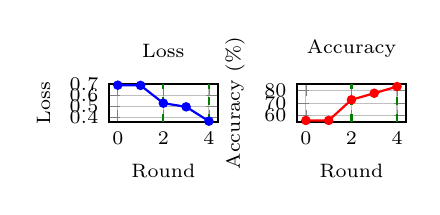
\begin{tikzpicture}
\begin{groupplot}[group style={group size=2 by 1}, xlabel={Round}]
\nextgroupplot[title={Loss}, ylabel={Loss}, ymin=0.36, ymax=0.70]
\addplot[blue, mark=*] coordinates {(0,0.691) (1,0.689) (2,0.529) (3,0.496) (4,0.367)};
\addplot[green!50!black, dashed] coordinates {(2,0.36) (2,0.70)};
\addplot[green!50!black, dashed] coordinates {(4,0.36) (4,0.70)};

\nextgroupplot[title={Accuracy}, ylabel={Accuracy (\%)}, ymin=55, ymax=85]
\addplot[red, mark=*] coordinates {(0,56.2) (1,56.2) (2,72.6) (3,77.8) (4,83.1)};
\addplot[green!50!black, dashed] coordinates {(2,55) (2,85)};
\addplot[green!50!black, dashed] coordinates {(4,55) (4,85)};
\end{groupplot}
\end{tikzpicture}
\caption{Async FL with $K=2$ under IID partitioning.}
\label{fig:async_k2_iid}
\end{figure}

\begin{figure}[!t]
\centering
\input{Tikz-Figs/fig_async_k2_noniid}
\caption{Async FL with $K=2$ under non-IID partitioning.}
\label{fig:async_k2_noniid}
\end{figure}

For $K=4$, upload reduction increases to 74.55\%, but accuracy decreases to 79.21\% under IID and 83.89\% under non-IID. Fig.~\ref{fig:async_k4_iid} and Fig.~\ref{fig:async_k4_noniid} show extended plateaus during shallow-only rounds, followed by sharp improvements when deep updates occur. This behavior reflects increased staleness in deep parameters, which slows convergence and reduces final accuracy.

\begin{figure}[!t]
\centering
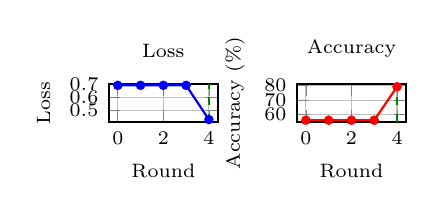
\begin{tikzpicture}
\begin{groupplot}[group style={group size=2 by 1}, xlabel={Round}]
\nextgroupplot[title={Loss}, ylabel={Loss}, ymin=0.41, ymax=0.70]
\addplot[blue, mark=*] coordinates {(0,0.691) (1,0.691) (2,0.691) (3,0.691) (4,0.428)};
\addplot[green!50!black, dashed] coordinates {(4,0.41) (4,0.70)};

\nextgroupplot[title={Accuracy}, ylabel={Accuracy (\%)}, ymin=55, ymax=81]
\addplot[red, mark=*] coordinates {(0,56.2) (1,56.2) (2,56.2) (3,56.2) (4,79.2)};
\addplot[green!50!black, dashed] coordinates {(4,55) (4,81)};
\end{groupplot}
\end{tikzpicture}
\caption{Async FL with $K=4$ under IID partitioning.}
\label{fig:async_k4_iid}
\vspace{-0.2cm}
\end{figure}

\begin{figure}[!t]
\centering
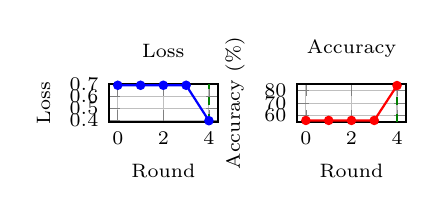
\begin{tikzpicture}
\begin{groupplot}[group style={group size=2 by 1}, xlabel={Round}]
\nextgroupplot[title={Loss}, ylabel={Loss}, ymin=0.39, ymax=0.70]
\addplot[blue, mark=*] coordinates {(0,0.691) (1,0.691) (2,0.691) (3,0.691) (4,0.400)};
\addplot[green!50!black, dashed] coordinates {(4,0.39) (4,0.70)};

\nextgroupplot[title={Accuracy}, ylabel={Accuracy (\%)}, ymin=55, ymax=85]
\addplot[red, mark=*] coordinates {(0,56.2) (1,56.2) (2,56.2) (3,56.2) (4,83.9)};
\addplot[green!50!black, dashed] coordinates {(4,55) (4,85)};
\end{groupplot}
\end{tikzpicture}
\caption{Async FL with $K=4$ under non-IID partitioning.}
\label{fig:async_k4_noniid}
\vspace{-0.2cm}
\end{figure}

\subsection{Discussion of Results}
\begin{table}[!t]
\centering
\caption{Summary of experimental results. $^{\dagger}$~mean $\pm$ standard deviation over three random seeds; all other rows are single runs. Upload is measured on the full \texttt{state\_dict} for both arms, and the centralized row is a non-federated reference rather than an upper bound.}
\label{tab:summary}
\small
\setlength{\tabcolsep}{4pt}
\begin{tabular}{@{}lccc@{}}
\toprule
\textbf{Experiment} & \textbf{Acc. (\%)} & \textbf{Upload (MiB)} & \textbf{Red.} \\
\midrule
Centralized & 84.08 & -- & -- \\
\midrule
Sync IID$^{\dagger}$ & $82.68 \pm 0.98$ & 1699.75 & 0.00\% \\
Sync non-IID & 84.53 & 1699.75 & 0.00\% \\
\midrule
Async $K=1$ IID & 83.71 & 1699.75 & 0.00\% \\
Async $K=2$ IID$^{\dagger}$ & $83.18 \pm 0.76$ & 855.01 & 49.70\% \\
Async $K=4$ IID & 79.21 & 432.64 & 74.55\% \\
Async $K=2$ non-IID & 84.62 & 855.01 & 49.70\% \\
Async $K=4$ non-IID & 83.89 & 432.64 & 74.55\% \\
\bottomrule
\end{tabular}
\end{table}
Upload volume is measured identically for both schedules, as the serialized size of the full \texttt{state\_dict}. Counting only trainable parameters omits the BatchNorm running statistics, which are transmitted but carry no gradient, understating each model by 3{,}872 bytes and a four-round, three-client run by 46{,}464 bytes. That is the entire apparent difference between the synchronous and $K=1$ configurations; under a single convention the two are identical, as they must be, since $K=1$ is synchronous FedAvg in communication terms.

Table~\ref{tab:summary} summarizes the results. Three key observations emerge. First, accuracy gains are temporally aligned with rounds that include deep parameter updates. Second, $K=2$ provides the best trade-off, achieving nearly 50\% reduction in upload cost while maintaining accuracy close to synchronous FL. Third, accuracy differences between synchronous FedAvg and asynchronous $K=2$ under IID partitioning are small relative to seed-to-seed variation. Over three seeds the synchronous baseline alone spans 1.91 percentage points (81.85\% to 83.76\%), which is wider than the mean paired difference of $+0.50$ percentage points between the two schedules ($p=0.31$). The asynchronous schedule is at least as accurate on every seed tested, but the margin is small and dominated by a single seed. The scheduling change is therefore best characterised as accuracy-neutral at this federation size rather than accuracy-improving, and the communication saving is obtained without a measurable accuracy penalty. The single non-IID pair (84.62\% versus 84.53\%) is consistent with this reading but, being one run per configuration, does not by itself establish robustness under heterogeneity.

The $K=1$ row is algorithmically identical to synchronous FedAvg, yet Table~\ref{tab:summary} reports a different accuracy; the two differ only in the floating-point precision used to accumulate the aggregation. From bitwise identical initial parameters on identical partitions they diverge by a maximum relative difference of $1.3 \times 10^{-7}$ after one round, which is float32 machine epsilon, yet finish $1.86$ percentage points apart. With four rounds the model is far from converged and such perturbations are amplified rather than damped. This is the same effect that produces the seed-to-seed spread above, and it is why we treat the accuracy column as indicative and rest our claims on the communication column.

Several limitations bound these results. The federation comprises three clients over four rounds with one local epoch per round, which is small relative to deployed FL systems. The layer partition is fixed a priori and the interval $K$ is constant, with no adaptation to observed layer discrepancy. The shallow group holds only $0.60\%$ of model parameters, so shallow-only rounds carry limited information and the upload saving derives almost entirely from omitting the deep group; this also highlights the need for more balanced partitions or adaptive scheduling in future work. Accuracy is replicated over three seeds only for the IID synchronous and $K=2$ configurations; the non-IID and $K=4$ results are single runs and should be read as indicative. Finally, only upload volume was measured. Energy, latency, and congestion benefits are inferred from reduced transmission volume rather than observed, and are stated as potential system-level consequences.



\section{Conclusion}

In this paper we characterized a fixed-schedule form of layer-wise update scheduling for communication-efficient federated learning on IoT health devices. By partitioning model parameters into shallow and deep groups by parameter mass and synchronizing them at different fixed frequencies, the method reduces uplink communication without architectural modification, without runtime measurement of layer statistics, and without any server-side per-layer state. It therefore applies directly on top of standard FedAvg, which is the property that matters most for severely resource-constrained deployments.

Evaluation on PTB-XL ECG classification demonstrates that $K=2$ achieves a 49.70\% reduction in client upload volume with no accuracy penalty measurable at three seeds, while $K=4$ increases the reduction to 74.55\% at a clear cost in accuracy. The upload reductions are exact consequences of the schedule and the layer partition, and are therefore independent of the seed; the accuracy comparison is not, and is reported with its seed variance.

Several directions remain open. Our evaluation does not include hardware deployment with direct power and latency measurement, a formal convergence analysis under bounded deep-layer staleness, adaptive or learned selection of $K$ and of the layer grouping, or comparison against gradient compression and split-learning baselines \cite{vepakomma2018}. Extending the evaluation to larger federations, additional architectures, and additional datasets is likewise left to future work.

Overall, the proposed approach provides a simple and practical mechanism for balancing communication efficiency and learning performance in resource-constrained FL deployments.

%\section*{Acknowledgment}


\bibliographystyle{IEEEtran}
\bibliography{ref}


% \begin{thebibliography}{10}

% \bibitem{mcmahan2017}
% B. McMahan, E. Moore, D. Ramage, S. Hampson, and B. A. y Arcas, ``Communication-efficient learning of deep networks from decentralized data,'' in \textit{Proc. AISTATS}, 2017, pp. 1273--1282.

% \bibitem{yang2019}
% Q. Yang, Y. Liu, T. Chen, and Y. Tong, ``Federated machine learning: Concept and applications,'' \textit{ACM Trans. Intell. Syst. Technol.}, vol. 10, no. 2, pp. 1--19, 2019.

% \bibitem{konecny2016}
% J. Konečný, H. B. McMahan, D. Ramage, and P. Richtárik, ``Federated optimization: Distributed machine learning for on-device intelligence,'' \textit{arXiv preprint arXiv:1610.02527}, 2016.

% \bibitem{hartmann2018}
% M. Hartmann, ``Federated learning,'' Master's thesis, Technical University of Munich, 2018.

% \bibitem{yuan2020}
% X. Yuan, J. Chen, N. Zhang, et al., ``SplitFed learning without sharing raw data for privacy-preserving federated learning in healthcare IoT,'' \textit{IEEE Internet Things J.}, vol. 8, no. 16, pp. 13 351--13 358, 2020.

% \bibitem{tariq2024}
% M. A. Tariq et al., ``Trustworthy federated learning: A survey,'' \textit{arXiv preprint arXiv:2305.16424}, 2024.

% \bibitem{xie2019asynchronous}
% C. Xie, S. Koyejo, and I. Gupta, ``Asynchronous federated optimization,'' in \textit{Proc. OPT}, 2019.

% \bibitem{wagner2020}
% P. Wagner et al., ``PTB-XL, a large publicly available electrocardiography dataset,'' \textit{Sci. Data}, vol. 7, no. 1, p. 154, 2020.

% \bibitem{yosinski2014}
% J. Yosinski, J. Clune, Y. Bengio, and H. Lipson, ``How transferable are features in deep neural networks?'' in \textit{Proc. NeurIPS}, 2014, pp. 3320--3328.

% \bibitem{paszke2019}
% A. Paszke et al., ``PyTorch: An imperative style, high-performance deep learning library,'' in \textit{Proc. NeurIPS}, 2019, pp. 8024--8035.

% \end{thebibliography}

\end{document}